\documentclass[12pt]{article}

\usepackage{graphicx}
\usepackage{paralist}
\usepackage{amsfonts}
\usepackage{amsmath}
\usepackage{hhline}
\usepackage{booktabs}
\usepackage{multirow}
\usepackage{multicol}
\usepackage{url}

\oddsidemargin -10mm
\evensidemargin -10mm
\textwidth 160mm
\textheight 200mm
\renewcommand\baselinestretch{1.0}

\pagestyle {plain}
\pagenumbering{arabic}

\newcounter{stepnum}

%% Comments

\usepackage{color}

\newif\ifcomments\commentstrue

\ifcomments
\newcommand{\authornote}[3]{\textcolor{#1}{[#3 ---#2]}}
\newcommand{\todo}[1]{\textcolor{red}{[TODO: #1]}}
\else
\newcommand{\authornote}[3]{}
\newcommand{\todo}[1]{}
\fi

\newcommand{\wss}[1]{\authornote{blue}{SS}{#1}}

\title{Assignment 4, Design Specification}
\author{Boming Jin jinb5}

\begin{document}

\maketitle
This Assignment4 specification contains modules, types, and methods for implementing the classic game \textit{2048}. When starting the game.
Users can simply press "w" "a" "s" "d" on the keyboard to slide all numbers on the board with one direction per sliding. 
Numbers can be slid vertically or horizontally. Boards will generate two numbers initially (which is 2 or 4) within random positions,
also, after each sliding, the board will spawn a number 2 or 4 randomly. Users need to slide those numbers and add the same numbers together
to get a final goal which is 2048. There is only one way about losing the game --- when the board is full of numbers and there is no more
possible moving, then users will fail this round. To simply run the game, just use "make demo" in the terminal to run the game.

\begin{center}
  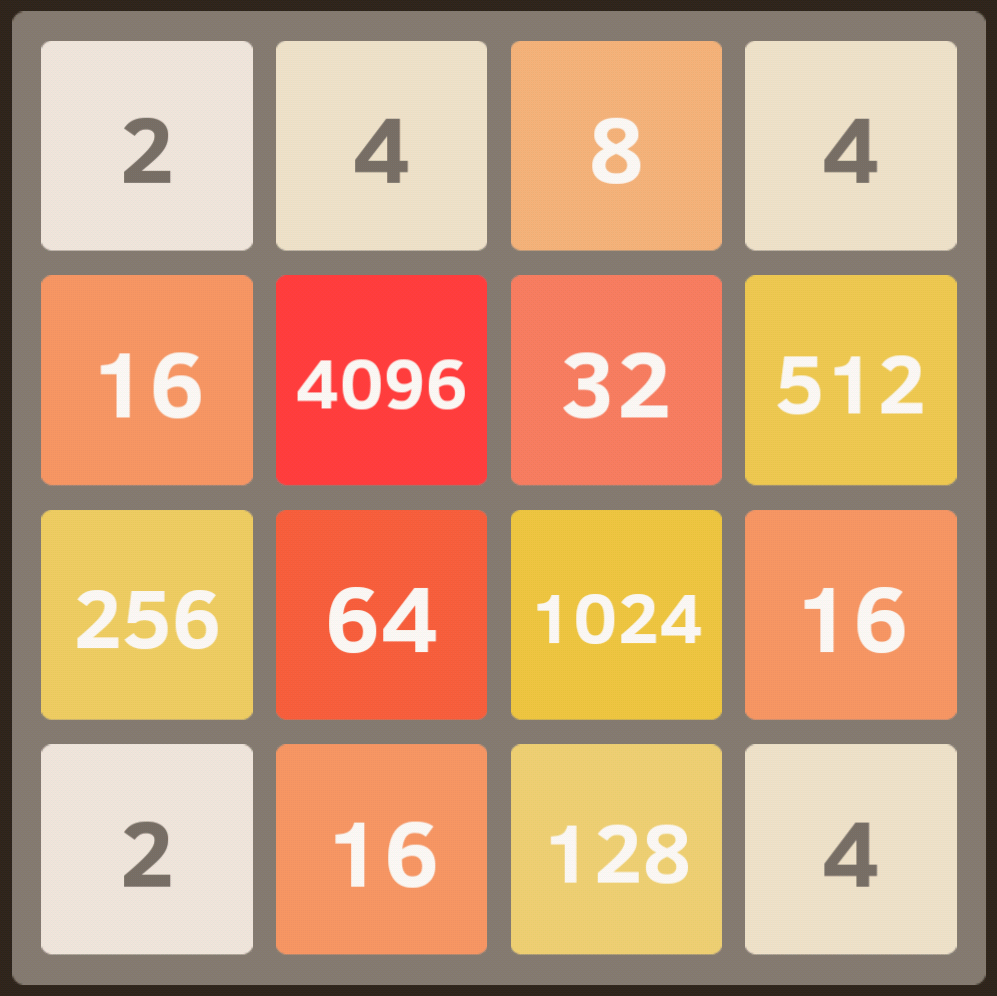
\includegraphics[width=0.5\textwidth]{2048.png}

  Picture found on Google
\end{center}

\newpage

\section{Overview of the design}

My design applies Model View Controller(MVC) design pattern, Singleton Design pattern. The \textit{gameController} (controller),
\textit{BoardT} (model), \textit{userInterface} (view) composed MVC. The MVC design pattern was designed as the following path: 
my \textit{StatusT} moudle stores states of cell in the board, and \textit{BoardT} module uses \textit{StatusT} as the state variables
then manipulate the status of each cell of the board. My \textit{userInterface} module built for display any information of the game in
text version. The \textit{gameController} module is for controlling the input and the output actions. 

\medskip
For getInstance() method in both \textit{gameController} and \textit{userInterface}, it is in order to obtain an abstract object during
the running time. 

\bigskip

\noindent A UML diagram for the architecture of my classes

\medskip

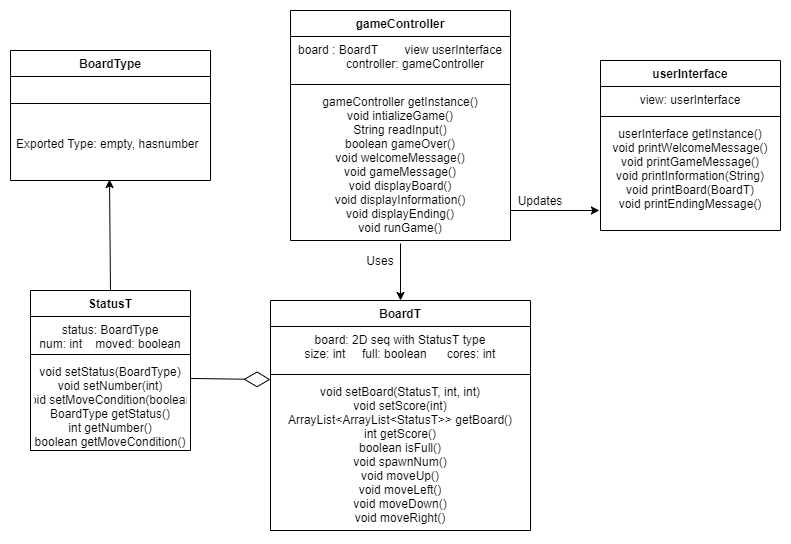
\includegraphics[width=0.9\textwidth]{A4UML.png}

\newpage

\subsection*{Likely Changes my design considers:}

\begin{itemize}
  \item Grid size for harder level of the game \textit{2048}
  \item Some good GUI for users to play game comfortably
  \item Multiple operations for operating the game (i.e. arrow keys to control the direction, mouse buttons to restart games, etc.)
  \item Store the best Score of the user
  \item Check how many moves that users did
  \item Rank scores for different users
\end{itemize}

\newpage

\section* {BoardType Module}

\subsection*{Module}

BoardType

\subsection* {Uses}

N/A

\subsection* {Syntax}

\subsubsection* {Exported Constants}

None

\subsubsection* {Exported Types}

BoardType = \{empty, hasnumber\}

\medskip

\noindent \textit{//empty represent that the cell is 0(empty), hasnumber says that the cell has some number in it(i.e. 2, 4, 8, 16, ...)}

\subsubsection* {Exported Access Programs}

None

\subsection* {Semantics}

\subsubsection* {State Variables}

None

\subsubsection* {State Invariant}

None

\newpage

\section* {StatusT Module}

\subsection* {Module}

StatusT

\subsection*{Uses}

BoardType

\subsection* {Syntax}

\subsection*{Exported Constants}

None

\subsection*{Exported Types}

None

\subsubsection* {Exported Access Programs}

\begin{tabular}{| l | l | l | p{6cm} |}

\hline
\textbf{Routine name} & \textbf{In} & \textbf{Out} & \textbf{Exceptions}\\
\hline
StatusT & BoardType, $\mathbb{N}$ & BoardT & \\
\hline
setStatus & BoardType &  & \\
\hline
setNumber & $\mathbb{N}$ &  & \\
\hline
setMoveCondition & $\mathbb{B}$ & & \\
\hline
getStatus &  & BoardType & \\
\hline
getNumber &  & $\mathbb{N}$ & \\
\hline
getMoveCondition &  & $\mathbb{B}$ & \\
\hline
 
\end{tabular}

\subsection* {Semantics}

\subsection*{State Variables}

status: BoardType \\
num: $\mathbb{N}$ \\
moved: $\mathbb{B}$ \\
\noindent \textit{//status represent if the current cell is empty or not, num represents the number that this cell stored, 
                  \textit{moved} represent if the current cell been moved in one user's action(without this will add all numbers together in one action 
                  i.e. 0 2 2 4 turns to 0 0 0 8 when the user only slides the board to the right once)}

\subsection*{State Invariant}

None

\subsection*{Assumptions}

When initializing a new StatusT as the cell of the board, I assume those cells not moved(moved by users, like slide to right, etc.)

\subsubsection* {Access Routine Semantics}

new StatusT(t, i):

\begin{itemize}
  \item transition: status, num $:=$ t, i \quad //BoardType t, int i
  \item output: out $:=$ self 
\end{itemize}

\noindent setStatus(t):

\begin{itemize}
  \item transition: status $:=$ t \quad //BoardType t
  \item exception: none
\end{itemize}

\noindent setNumber(i):

\begin{itemize}
  \item transition: num $:=$ i
  \item exception: none
\end{itemize}

\noindent setMoveCondition(b):

\begin{itemize}
  \item transition: moved $:=$ b
  \item exception: none
\end{itemize}

\noindent getStatus():

\begin{itemize}
  \item output: out $:=$ status
  \item exception: none
\end{itemize}

\noindent getNumber():

\begin{itemize}
  \item output: out $:=$ num
  \item exception: none
\end{itemize}

\noindent getMoveCondition():

\begin{itemize}
  \item output: out $:=$ moved
  \item exception: none
\end{itemize}


\newpage

\section* {BoardT Module}

\subsection* {Module}

BoardT

\subsection*{Uses}

StatusT

\subsection* {Syntax}

\subsection*{Exported Constants}

size of the seq of (seq of StatusT) = 4 \quad //Size of the board is 4 x 4

\subsection*{Exported Types}

None

\subsubsection* {Exported Access Programs}

\begin{tabular}{| l | l | l | p{6cm} |}
\hline
\textbf{Routine name} & \textbf{In} & \textbf{Out} & \textbf{Exceptions}\\
\hline
BoardT &  & BoardT & \\
\hline
BoardT & seq of (seq of StatusT) & BoardT & \\
\hline
setBoard & StatusT, $\mathbb{N}$, $\mathbb{N}$ &  & \\
\hline
setScore & $\mathbb{N}$ &  & \\
\hline
getBoard &  & seq of (seq of StatusT) & \\
\hline
getScore &  & $\mathbb{N}$ & \\
\hline
isFull &  & $\mathbb{B}$ & \\
\hline
moveUp &  &  & \\
\hline
moveLeft &  &  & \\
\hline
moveDown &  &  & \\
\hline
moveRight &  &  & \\
\hline

\end{tabular}

\subsection* {Semantics}

\subsection*{State Variables}

board: seq of (seq of StatusT) \\
full: $\mathbb{B}$ \\
score : $\mathbb{N}$ 

\subsection*{State Invariant}

None

\subsection*{Assumptions}

Assume when running the game, construct BoardT at first before other operations.
\newline
When initializing will spawn 2 numbers(2 or 4) in random positions of the board(by using a local function) and the number of others is 0(empty).
This means the status of StatusT is empty, and the number of StatusT is 0.
\newline
Assume there is a \textit{Random()} function get the random numbers that I want.

\subsubsection* {Access Routine Semantics}

new BoardT():

\begin{itemize}
  \item transition: board, score, full $:=$ seq[4] of (seq[4] of StatusT), 0, false
  \item output: out $:=$ self
  \item exception: none
\end{itemize}

\noindent new BoardT(b):

\begin{itemize}
  \item transition: board, score, full $:=$ b, 0, false \quad // b is seq[4] of (seq[4] of StatusT)
  \item output: self
  \item exception: none
\end{itemize}

\noindent setBoard(s, r, c):
\begin{itemize}
  \item transition: board[r][c] $:=$ s \\
   \quad //s is StatusT. r, c are the target position of the board that we want to set(i.e. board[0][0] is the left top corner of the board)
  \item exception: none
\end{itemize}

\noindent setScore(s):
\begin{itemize}
  \item transition: score $:=$ s \quad //s is the integer number
  \item exception: none
\end{itemize}

\noindent getBoard():
\begin{itemize}
  \item output: out $:=$ seq[4] of (seq[4] of StatusT)
  \item exception: none
\end{itemize}

\noindent getScore():
\begin{itemize}
  \item output: out $:=$ score
  \item exception: none
\end{itemize}

\noindent isFull():
\begin{itemize}
  \item output: out $:=$ ($\forall x, y : \mathbb{N}$ $|$ $x \in [0...size - 1] \land y \in [0...size - 1]$ $:$ board[x][y] $!=$ 0) \quad //if all cells of the board have number then the board is full
  \item exception: none
\end{itemize}

\noindent moveUp():
\begin{itemize}
  \item transition: board $:=$ ($\forall x, y : \mathbb{N}$ $|$ $x \in [1...size - 1] \land y \in [0...size - 1]$ $:$ move("w", x, y, \{true, false\})) \\
  \noindent \textit{//when moving(moveUp(), moveRight(), etc.), will use this local function \textit{move()} twice for reset the moved status for StatusT.
                      if state x before y then that means using for loop for x first then using for loop for y, vice versa}
  \item exception: none
\end{itemize}

\noindent moveLeft():
\begin{itemize}
  \item transition: board $:=$ ($\forall y, x : \mathbb{N}$ $|$ $y \in [1...size - 1] \land x \in [0...size - 1]$ $:$ move("w", x, y, \{true, false\}))
  \item exception: none
\end{itemize}

\noindent moveDown():
\begin{itemize}
  \item transition: board $:=$ ($\forall x, y : \mathbb{N}$ $|$ $x \in [size - 2...0] \land y \in [0...size - 1]$ $:$ move("w", x, y, \{true, false\}))
  \item exception: none
\end{itemize}

\noindent moveDown():
\begin{itemize}
  \item transition: board $:=$ ($\forall y, x : \mathbb{N}$ $|$ $y \in [size - 2...0] \land x \in [0...size - 1]$ $:$ move("w", x, y, \{true, false\}))
  \item exception: none
\end{itemize}

\subsubsection* {Local Functions}
\begin{itemize}
  \item spawnNum() $equiv$ ($x, y : \mathbb{N}$ $|$ $x = Random(0 - 3) \land y = Random(0 - 3)$ $:$ board.get(x).set(y, StatusT)) \\
  \noindent \textit{//Generate number in random cells of the board by using \textit{Random()} function, also if board.isFull() == true, then don't spawn new numbers}

  \item move(String s, int x, int y, boolean moved) \\
  \noindent \textit{//when using this local function we are moving cells, for example, if we are moving up, then cells will move from up to down and move in the up direction one by one, other directions are similar to moving up with different directions}

  \item swap: $StatusT \times StatusT \rightarrow StatusT \times StatusT $
  \newline
  \noindent swap(current, next) $\equiv$ \\
  ($\neg(current.number = 0) \land (next.number = 0) \rightarrow (next.number = current.number) \land (current.number = 0)$ \\
  $|$ $\neg(current.number = 0) \land \neg(next.number = 0) \land (current.moved = false) \land (next.moved = false) \rightarrow \\
  ((current.number = next.number) \rightarrow (next.number = 2 * current.number) \land (current.number = 0))$) \\
  \noindent \textit{//if the number of the current position is not 0 and the number of the next position is 0 then we swap the position of these two cells} \\
  \noindent \textit{//if the number of the current position is not 0 and the number of the next position is not 0 and they are equal then double the number of the next position, the number of the current position will be 0}
\end{itemize}

\newpage

\section* {userInterface Module}

\subsection* {Module}

userInterface

\subsection*{Uses}

None

\subsection* {Syntax}

\subsection*{Exported Constants}

None

\subsection*{Exported Types}

None

\subsubsection* {Exported Access Programs}

\begin{tabular}{| l | l | l | p{6cm} |}
\hline
\textbf{Routine name} & \textbf{In} & \textbf{Out} & \textbf{Exceptions}\\
\hline
getInstance &  & userInterface & \\
\hline
printWelcomeMessage &  &  & \\
\hline
printGameMessage &  &  & \\
\hline
printInformation &  &  & \\
\hline
printBoard & BoardT &  & \\
\hline
printEndingMessage &  &  & \\
\hline
\end{tabular}

\subsection* {Semantics}

\subsection*{Environment Variables}

window: part of screen to display everything related to the game

\subsection*{State Variables}


view: userInterface \\

\subsection*{State Invariant}

None

\subsection*{Assumptions}

Construct this object before running the game(before other classes use the method)

\subsubsection* {Access Routine Semantics}

getInstance():
\begin{itemize}
  \item transition: view $:=$ (view $=$ null $\rightarrow$ new userInterface())
  \item output: self
\end{itemize}

\noindent printWelcomeMessage():
\begin{itemize}
  \item transition: window $:=$ when user first time start the game or restart the game display this message
\end{itemize}

\noindent printGameMessage():
\begin{itemize}
  \item transition: window $:=$ tell the instruction of the game to users
\end{itemize}

\noindent printInformation():
\begin{itemize}
  \item transition: window $:=$ displays the information of the game to users(i.e. Score of the current round)
\end{itemize}

\noindent printBoard():
\begin{itemize}
  \item transition: window $:=$ displays the board which is consists of numbers to users, each cell is \textit{StatusT}, which stores the number
        of the cell. Numbers of cells could gotten by \textit{getNumber()} method in \textit{StatusT}. Note: board[x][y] is counting from
        left top corner.
\end{itemize}

\noindent printEndingMessage():
\begin{itemize}
  \item transition: window $:=$ displays the ending message of the game when users choose to exit the game
\end{itemize}

\newpage

\section* {gameController Module}

\subsection* {gameController Module}

\subsection* {Uses}

BoardT, userInterface

\subsection* {Syntax}

\subsubsection* {Exported Types}

None

\subsubsection* {Exported Constants}

None

\subsubsection* {Exported Access Programs}

\begin{tabular}{| l | l | l | p{6cm} |}
\hline
\textbf{Routine name} & \textbf{In} & \textbf{Out} & \textbf{Exceptions}\\
\hline
getInstance & BoardT, userInterface & gameController &  \\
\hline
initializeGame &  &  & \\
\hline
readInput &  & String & IllegalArgumentException \\
\hline
gameOver &  & $\mathbb{B}$ & \\
\hline
welcomeMessage &  &  & \\
\hline
gameMessage &  &  & \\
\hline
displayBoard &  &  & \\
\hline
displayInformation &  &  & \\
\hline
displayEnding &  &  & \\
\hline
runGame &  &  & \\
\hline
\end{tabular}

\subsection* {Semantics}

\subsection*{Environment Variables}

keypressed: Scanner // read the input of the user

\subsubsection* {State Variables}

board: BoardT
view: userInterface
controller: gameController

\subsubsection* {State Invariant}

None

\subsubsection* {Assumptions}

\textit{board} and \textit{view} already constructed before construct \textit{gameController}


\subsubsection* {Access Routine Semantics}

getInstance():
\begin{itemize}
  \item transition: controller $:=$ (controller = null $\Rightarrow$ new userInterface(board, view))
  \item output: self
\end{itemize}

\noindent initializeGame():
\begin{itemize}
\item transition: board $:=$ new BoardT()
\item output: none
\end{itemize}

\noindent readInput():
\begin{itemize}
\item output: keyboard $:$ String, scanned from terminal which is entered by users
\item exception: exc $:=$ (keyboard $\neq$ "w" $\land$ keyboard $\neq$ "a" $\land$ keyboard 
                           $\neq$ "s" $\land$ keyboard $\neq$ "d" $\land$ keyboard $\neq$ "r" $\land$ keyboard 
                           $\neq$ "e" $\rightarrow$ IllegalArgumentException) \\
\quad // "w", "a", "s", "d" represent for moving directions, "r" for restart the game, "e" for exit the game
\end{itemize}

\noindent gameOver():
\begin{itemize}
  \item output: ($\forall$ row of seq of number $\in$ board $:$ nextrow of seq of number $\neq$ row of seq of number) $\land$
                ($\forall$ column of seq of number $\in$ board $:$ nextcolumn of seq of number $\neq$ column of seq of number)
                $\rightarrow$ true
\end{itemize}

\noindent welcomeMessage():
\begin{itemize}
  \item transition: view $:=$ view.printWelcomeMessage()
\end{itemize}

\noindent gameMessage():
\begin{itemize}
  \item transition: view $:=$ view.printGameMessage()
\end{itemize}

\noindent displayBoard():
\begin{itemize}
  \item transition: view $:=$ view.printBoard(board)
\end{itemize}

\noindent displayInformation():
\begin{itemize}
  \item transition: view $:=$ view.printInformation()
\end{itemize}

\noindent displayEnding():
\begin{itemize}
  \item transition: view $:=$ view.printEndingMessage()
\end{itemize}

\noindent runGame():
\begin{itemize}
  \item transition: running the game, initialize board(game) first with welcome messages, then display the instruction, next let the user
                    play the game, at the end let the user have the power to decide to restart or end the game
\end{itemize}





\newpage

\section*{Critique of Design}

\begin{itemize}
  \item I choose to use StatusT to store the status of cells(i.e. if already moved in one action, numbers, if empty), which is convenient for
        me to combine multiple statuses, and easy to get or set for actually implementing. Also, the real condition of StatusT is hiding
        from other classes.
  \item Since I am only using controller and view modules once during the running time of the game, this offering fewer conflicts or unexpected state changes, 
        hence it was less hard to test and easier to find some logical bugs during implementing time.
  \item For StatusT I think it is not essential because I chose to offer an enum class to represent the empty condition of the cell, but it is more
        easier to use 0 as empty cells, so enum class BoardType might not necessary for this design. I could establish another enum class that is used
        to combine with users' inputs, for example, if the user press "w", then the enum value could be "UP", etc.
  \item My StatusT might not provide generality to this design, since it worked for BoardT only, in other words, if I am going to add some new
        features, for instance, design the level of the game, design GUI for this game, then StatusT might not helpful for new classes adding.
  \item My modules are minimal since I think this is more helpful for me to check states of every objects, and easy to implement. Reduces the chance of
        meeting conflicts.
  \item When testing BoardT, since numbers spawning randomly around the board, so it is not really convenient to teat moveUP() and other similar functions.
        So I choose to reset every number in BoardT to be 0. But this might not enough for testing. Since we might meet unexpected bugs with more numbers.
  \item I did not test gameController by using JUnit, since methods inside gameController are most from BoardT and userInterface, so I think gameController
        is not needed to be tested.
  \item I designed this game based on the idea of MVC. I found that MVC was really helpful for me to maintain the program and reduces the risk when changing some
        parts of the implementation. MVC basically could be separated into three parts: The model which handling the inside of the data, status, logic, etc. Also
        model encapsulates them. The Controller handles the interaction between users' inputs and reactions of the model(how the model behave with specific actions).
  \item By applying MVC to design the game, I think my modules could be said high cohesion and low coupling, since each module has related functionalities inside,
        and, each module looks mostly independent of others. This property guarantees to reduce the risk of changing little will impact many others.
  
\end{itemize}

\section*{Answers to Questions:}

Question1: \\

\begin{center}
  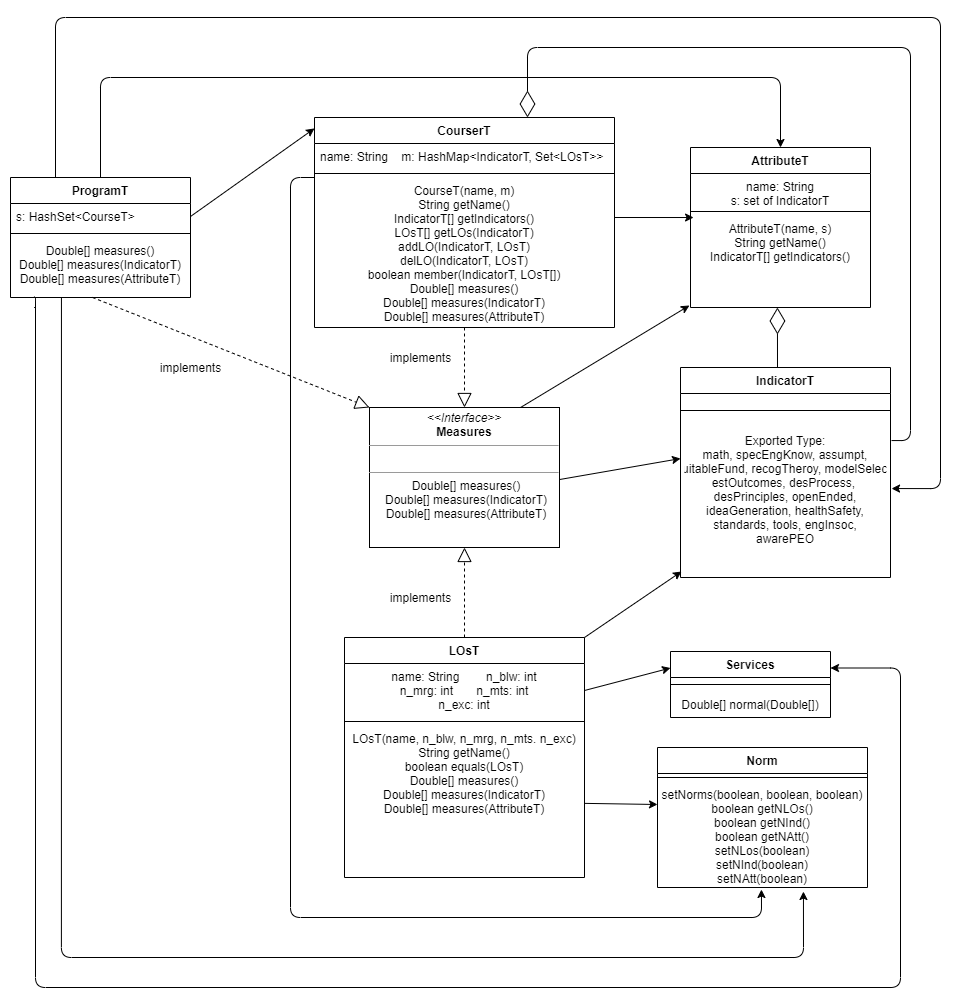
\includegraphics[width=0.8\textwidth]{A3UML.png}
\end{center}

\newpage

Question2: \\

\begin{center}
  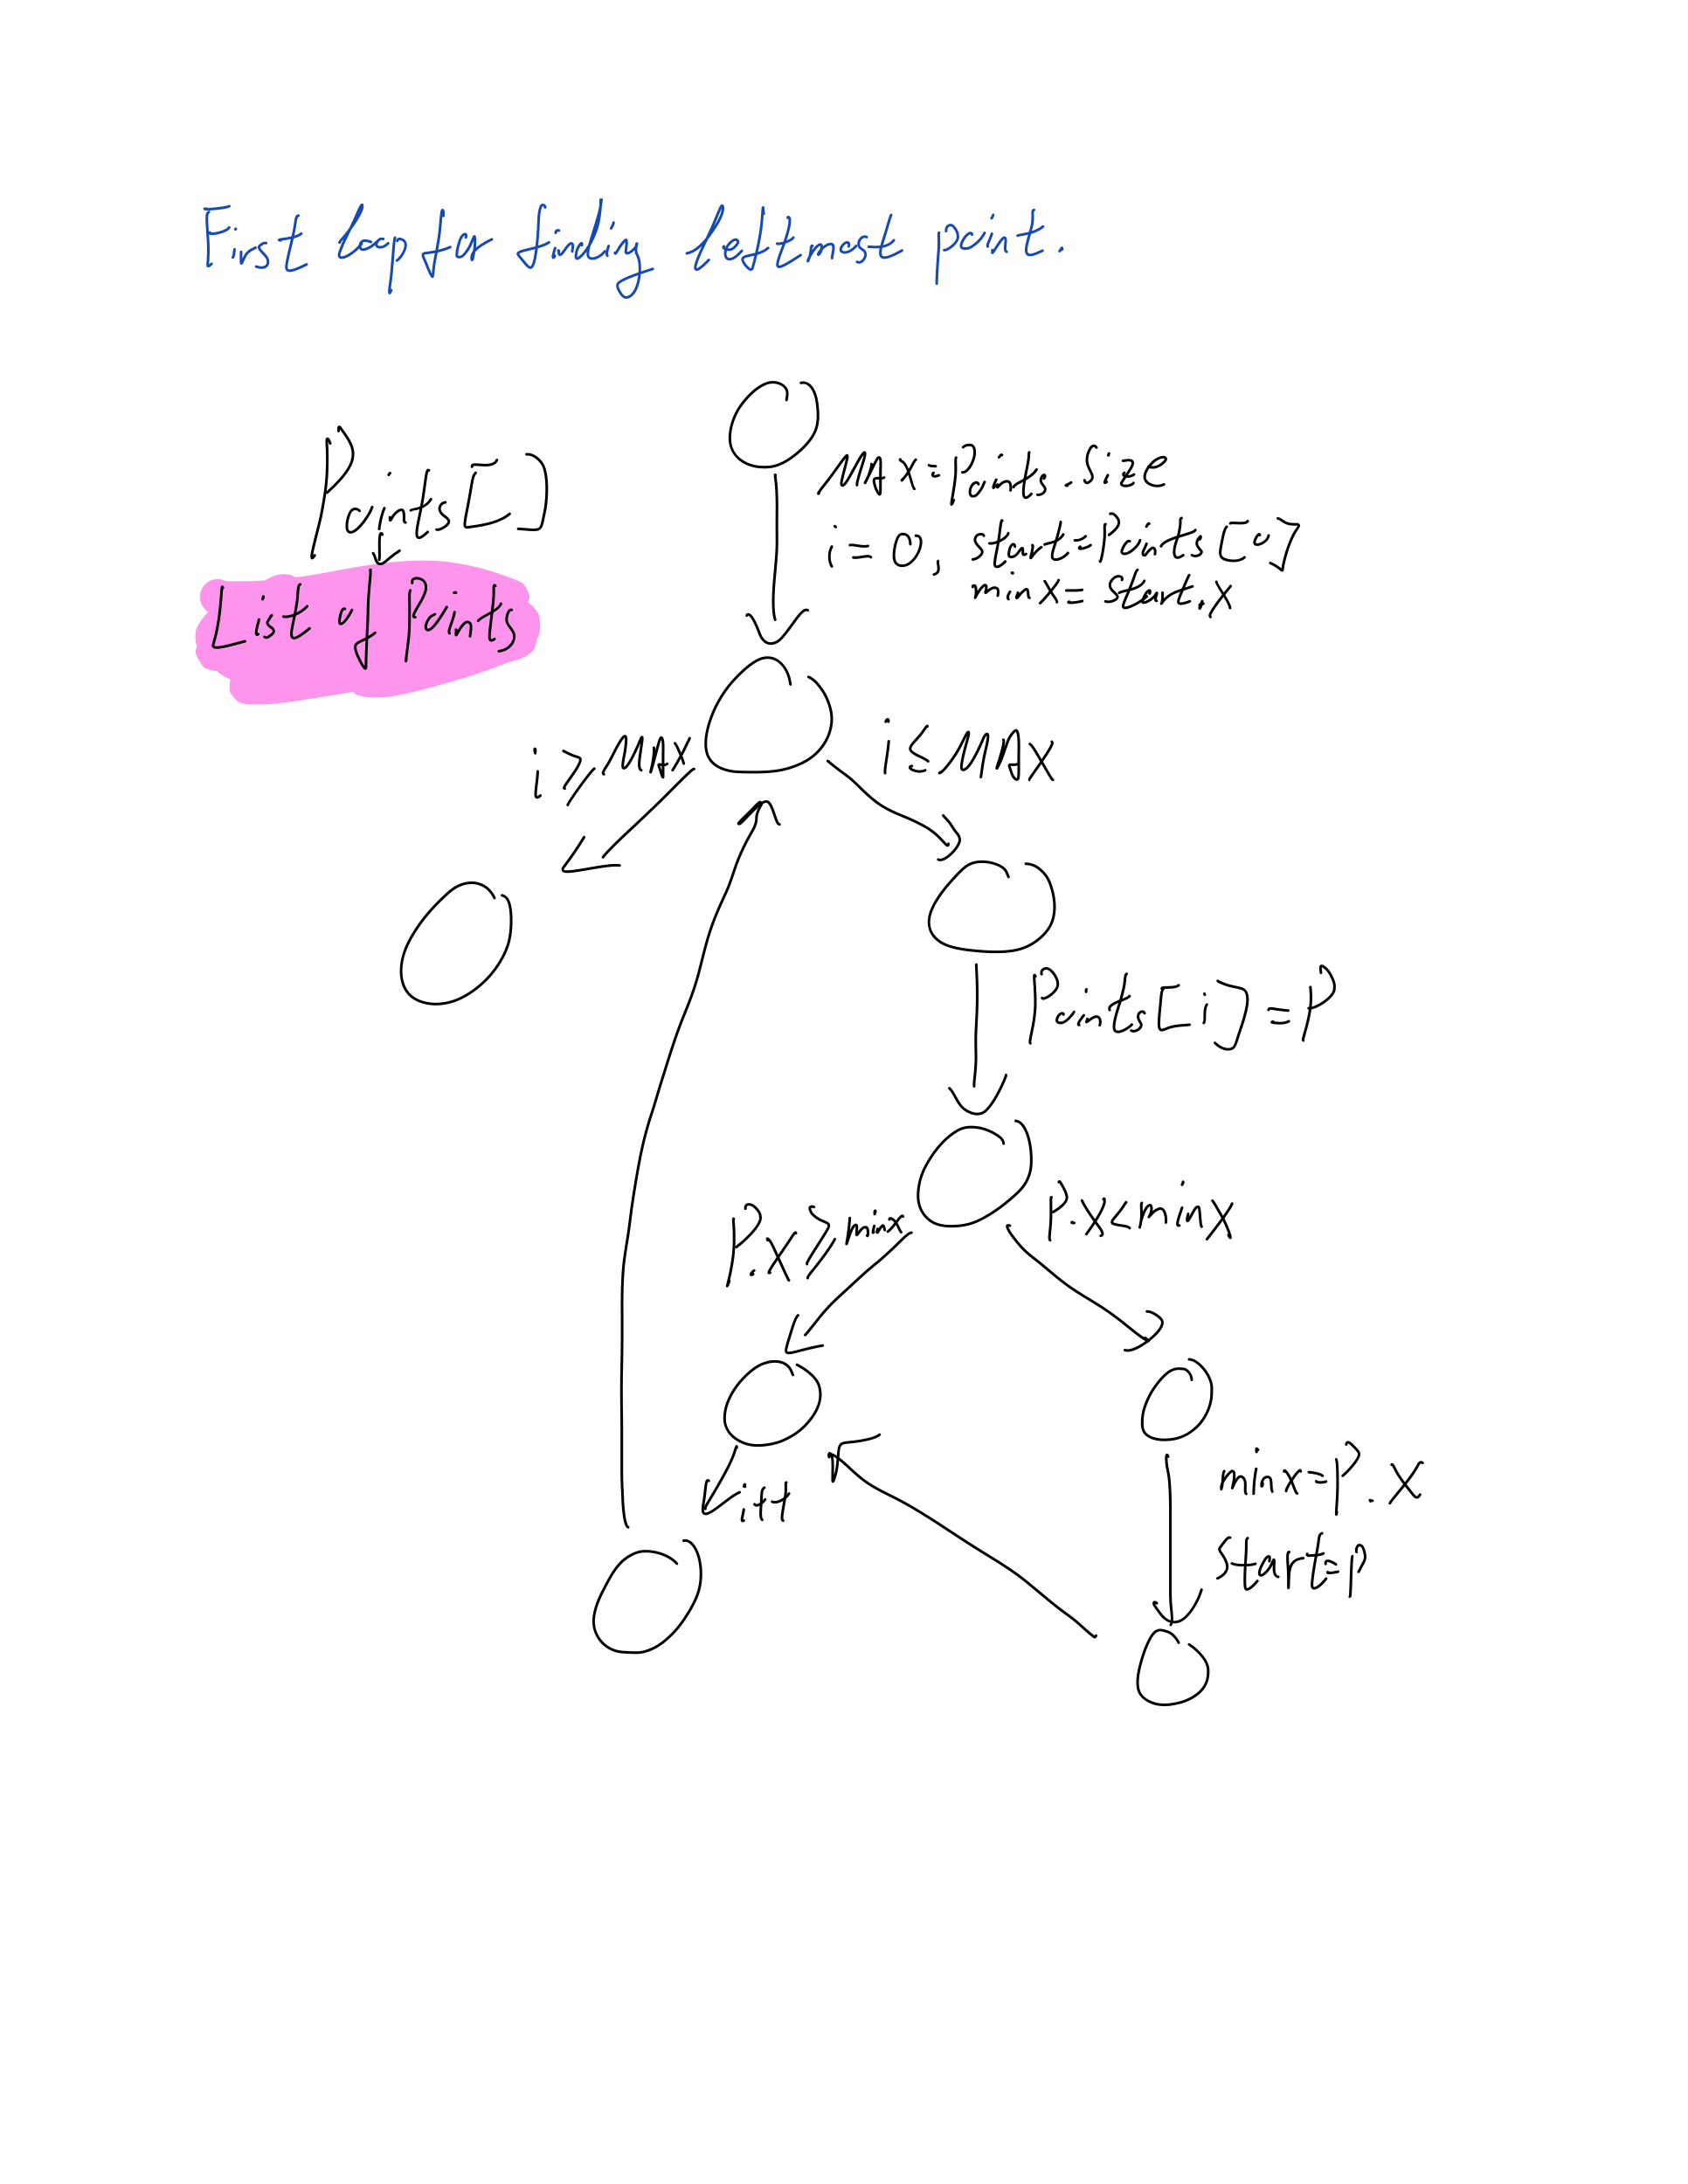
\includegraphics[width=0.9\textwidth]{Page1.png} \\
  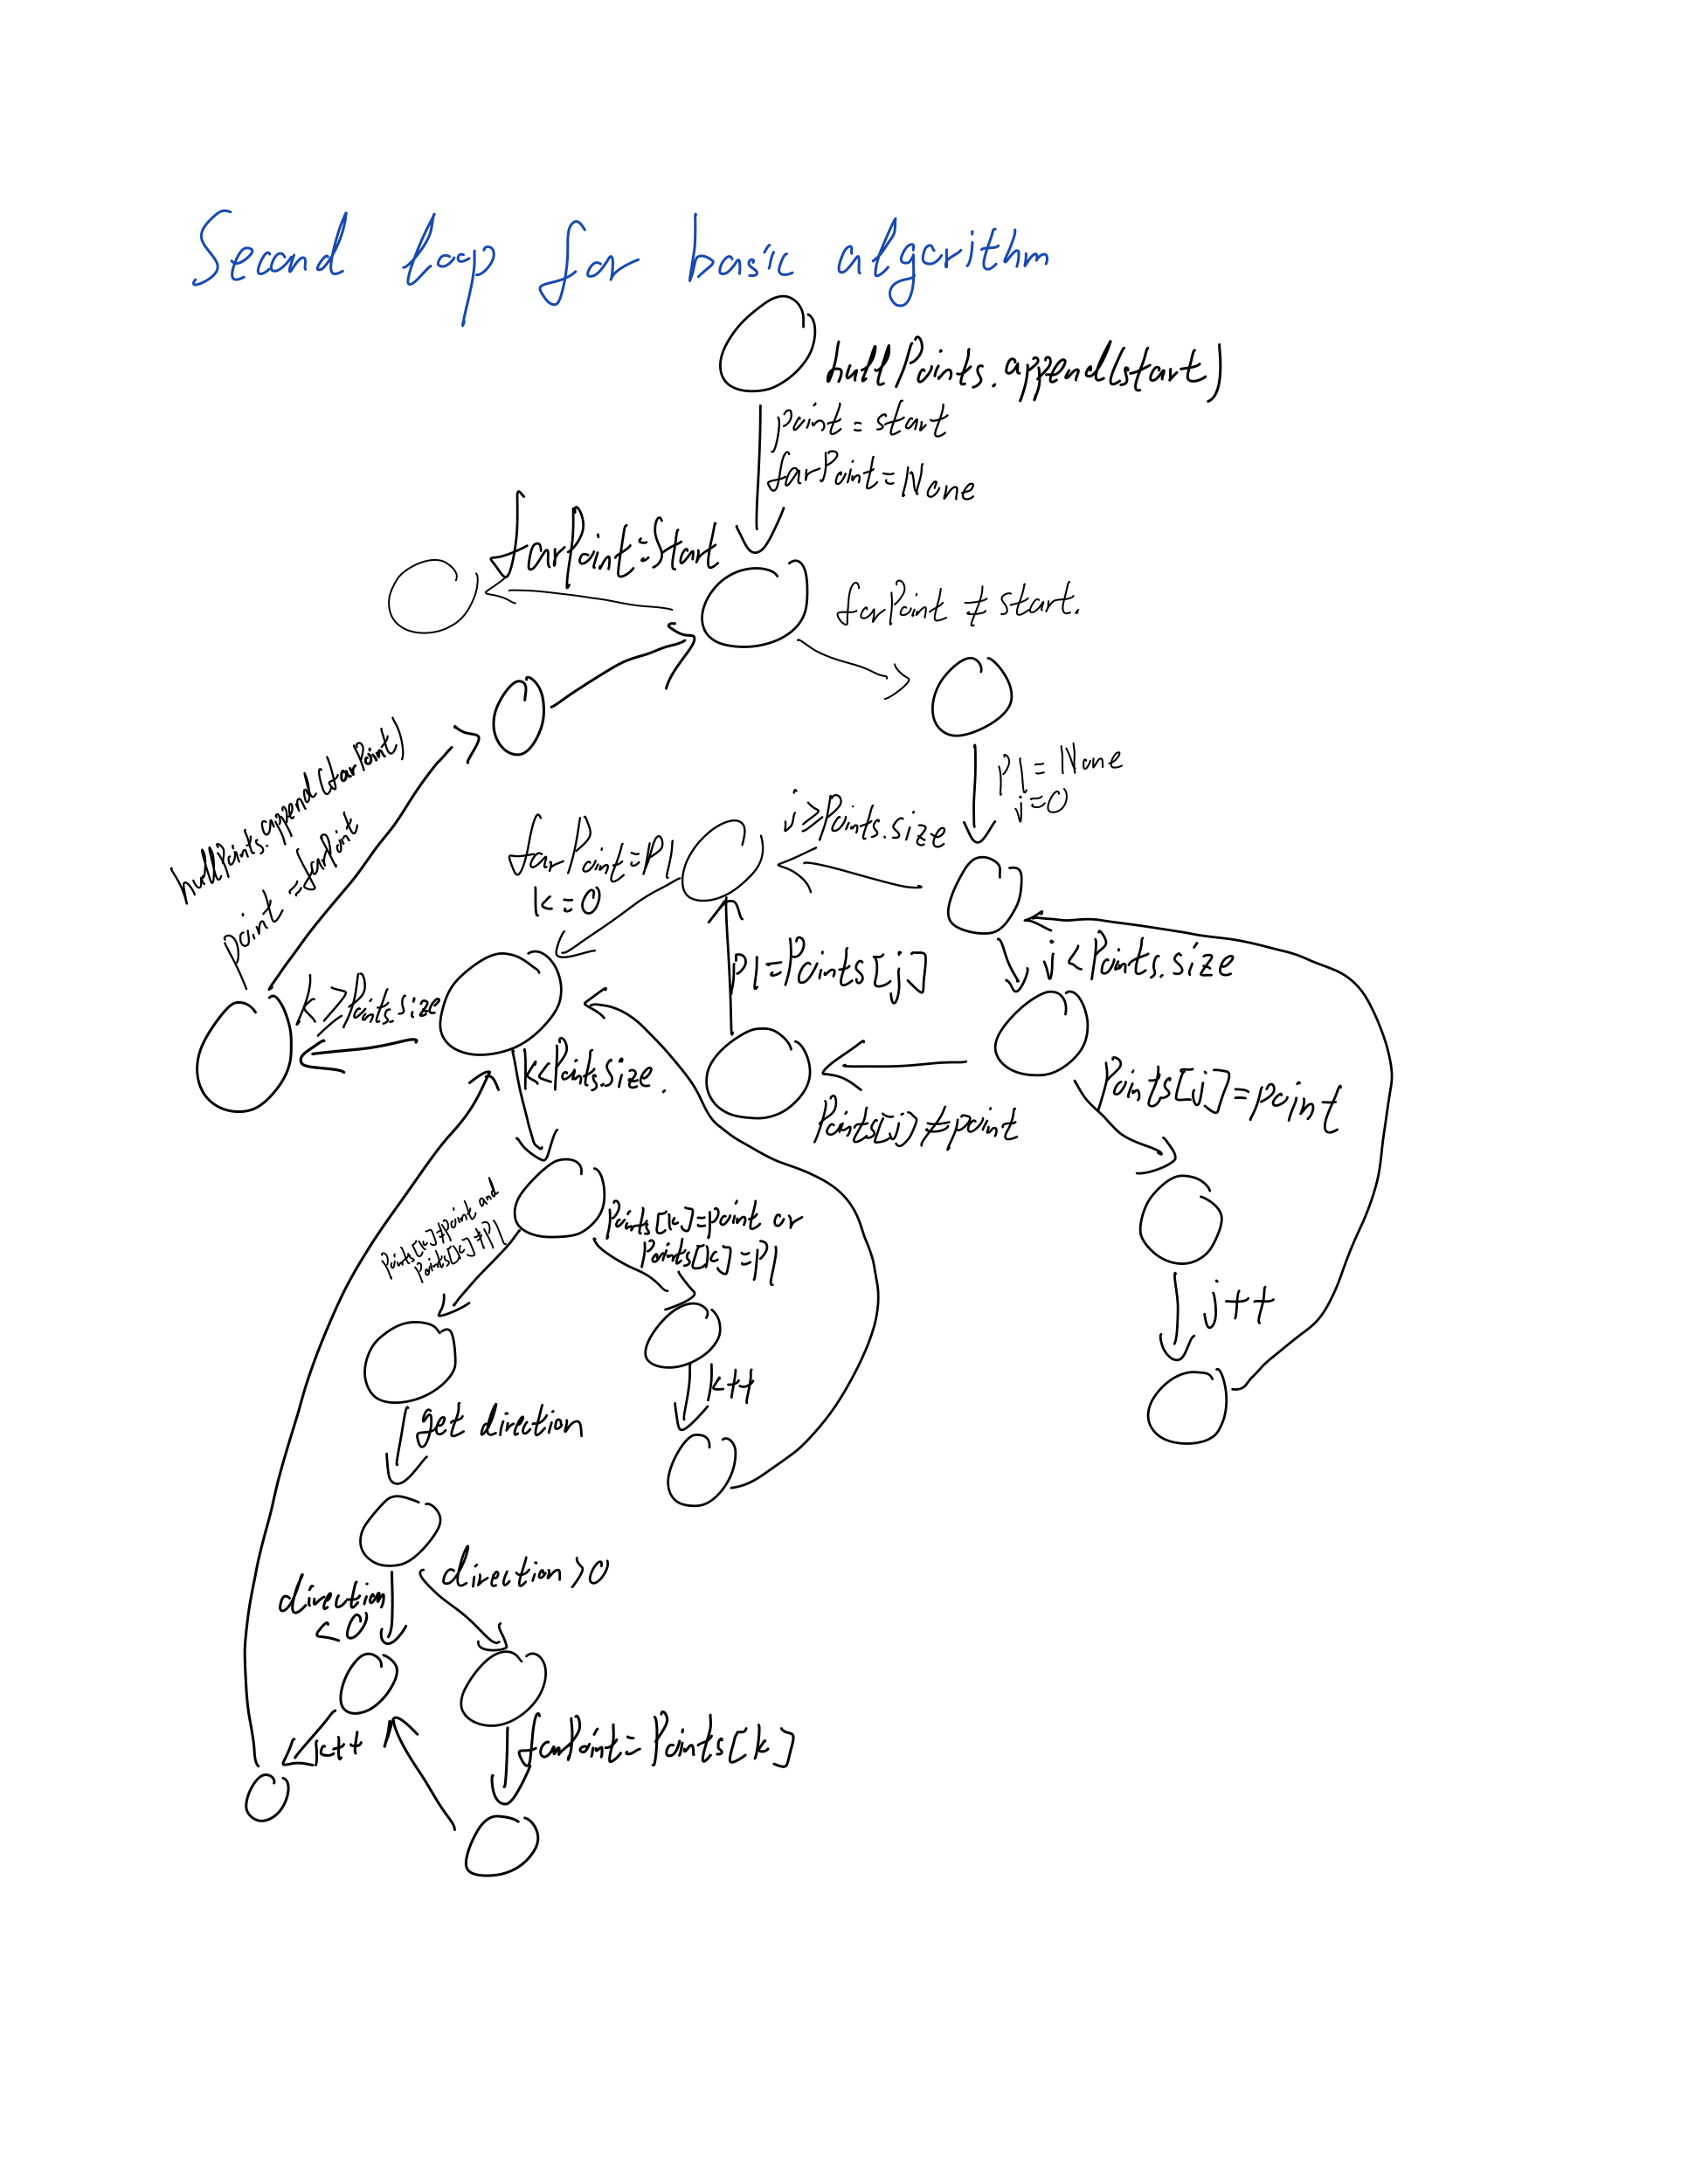
\includegraphics[width=1.2\textwidth]{Page2.png} \\
\end{center}

\end {document}